
\begin{His}


L'histoire des probabilités a commencé avec celle du hasard et notamment des jeux de hasard. Bien que quelques calculs de probabilité soient apparus dans des applications précises au Moyen Âge, ce n'est qu'au XVIIe siècle que la théorie des probabilités prend vraiment ses débuts. Elles évoluent sans vrai formalisme pendant deux siècles autour du célèbre problème des partis, de problèmes d'urnes ou d'autres problèmes issus de jeux. Apparaît alors la théorie classique des probabilités basée sur la théorie de la mesure et la théorie de l'intégration. Cette théorie s'est depuis lors diversifiée dans de nombreuses applications.

\vspace{0.4cm}
Les discussions entre scientifiques, la publication des ouvrages et leur transmission étant difficiles à certaines époques, certaines questions historiques restent difficiles à résoudre ; c'est le cas de la paternité de la théorie des probabilités.

\vspace{0.4cm}

\begin{wrapfigure}[11]{r}{3.6cm}
\vspace{-7mm}
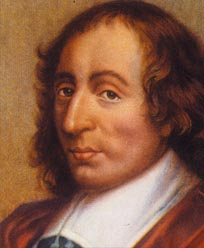
\includegraphics[scale=0.5]{image_chapitres/pascal.jpg}
\unnumberedcaption{Blaise \textsc{Pascal}}
\end{wrapfigure}

Le véritable début de la théorie des probabilités date de la correspondance entre Pierre de \textsc{Fermat} et Blaise \textsc{Pascal} en 1654 au sujet d'une désormais célèbre question posée par Antoine \textsc{Gombaud} (dit \textsc{chevalier de Méré}) : le problème des partis ou problèmes des points. 
\vspace{0.4cm}
«\textit{ Il avait pour objet de déterminer la proportion suivant laquelle l'enjeu doit être partagé entre les joueurs lorsqu'ils conviennent de ne point achever la partie, et qu'il leur reste à prendre pour la gagner, des nombres de points inégaux. Pascal en donna le premier la solution, mais pour le cas de deux joueurs seulement ; il fut ensuite résolu pour Fermat, dans le cas général d'un nombre quelconque de joueurs.} » (\textsc{Poisson}).
\vspace{0.4cm}
À la suite d'un séjour à Paris en 1655, Christian \textsc{Huygens} prend connaissance de cette discussion à l'Académie Parisienne et publie en 1657 le premier traité sur la théorie probabiliste : \textit{De ratiociniis in ludo aleae} (raisonnements sur les jeux de dés). C'est dans une lettre adressée à Frans van \textsc{Shooten}, qui a traduit son traité en latin dans \textit{Mathematische Oeffeningen}, qu'il attribue la paternité de la théorie des probabilités à \textsc{Pascal} et \textsc{Fermat} :

\vspace{0.4cm}

    « \textit{Il faut savoir d'ailleurs qu'il y a un certain temps que quelques-uns des plus Célèbres Mathématiciens de toute la France se sont occupés de ce genre de calcul, afin que personne ne m'attribue l'honneur de la première Invention qui ne m'appartient pas. }»

\vspace{0.4cm}

Puisqu'il fallait un certain délai entre l'écriture, la publication des œuvres et la diffusion de ces dernières, la paternité de la théorie des probabilités n'est pas unanime. Si la date de publication compte, c'est à \textsc{Huygens} que revient l'honneur d'être appelé le père de la théorie des probabilités, cependant si la date d'écrit compte, c'est à Jérôme \textsc{Cardan} que revient ce « titre ». Cependant la mauvaise réputation de \textsc{Cardan} a fait pencher la paternité sur \textsc{Pascal} et \textsc{Fermat}. \textsc{Leibniz} (1646-1716) ne cite que \textsc{Pascal}, \textsc{Fermat} et \textsc{Huygens} ; \textsc{Montmort} (1678-1719) cite \textsc{Cardan} mais d'une manière restrictive ; \textsc{Montucla} (1725-1799), \textsc{Laplace} (1749-1827) et \textsc{Poisson} (1781-1840) ne citent que \textsc{Pascal} et \textsc{Fermat}.

 
\PESP{https://fr.wikipedia.org/wiki/Histoire\_des_probabilit\%C3\%A9s}
 
\end{His}
